%%%%%%%%%%%%%%%%%%%%%%%%%%%%%%%%%%%%%%%%%%%%%%%%%%%%%%%%%%%%%%%%%%%%%%%%%%%%%%%%%%%%%%%%%%%%%%
%! Author = shenyixiao
%! Date = 2022/10/17
%Packages
%%%%%%%%%%%%%%%%%%%%%%%%%%%%%%%%%%%%%%%%%%%%%%%%%%%%%%%%%%%%%%%%%%
\documentclass[11pt, a4paper]{article}
\usepackage{graphicx}
\usepackage{fullpage}
\usepackage{hyperref}
\usepackage{listings}
\usepackage{appendix}
\usepackage{pdfpages}
\usepackage{color}
\usepackage{tocloft}        % This squashes the Table of Contents a bit
\usepackage{amsmath}
\usepackage{multirow}
\usepackage{tabularx}
\usepackage{caption}
\usepackage{subcaption}
%%%%%%%%%%%%%%%%%%%%%%%%%%%%%%%%%%%%%%%%%%%%%%%%%%%%%%%%%%%%%%%%%%%%%%%%%%%%%%%%%%%%%%%%%%%%%%
%Settings
%%%%%%%%%%%%%%%%%%%%%%%%%%%%%%%%%%%%%%%%%%%%%%%%%%%%%%%%%%%%%%%%%%
\setlength\cftbeforesecskip{3pt}
\setlength{\parskip}{4pt}        % sets spacing between paragraphs
\definecolor{MyLightYellow}{cmyk}{0,0.,0.2,0}
\interfootnotelinepenalty=500    % this prevents footnotes breaking across pages
\hypersetup{
	colorlinks=true,
	linkcolor=black,
	urlcolor=black,
	citecolor=black
}
\newcounter{mycounter}
\setcounter{mycounter}{0}


\begin{document}
%%%%%%%%%%%%%%%%%%%%%%%%%%%%%%%%%%%%%%%%%%%%%%%%%%%%%%%%%%%%%%%%%%%%%%%%%%%%%%%%%%%%%%%%%%%%
%Main
%%%%%%%%%%%%%%%%%%%%%%%%%%%%%%%%%%%%%%%%%%%%%%%%%%%%%%%%%%%%%%%%%%
\begin{center}
	\textbf{\large Drafts of Year 2 Project}
\end{center}

\begin{table}[!ht]
	\centering
	\begin{tabular}{|p{2cm}|p{2cm}|p{6cm}|}
		\hline
		Version1.0 & 4 Dec 2022
		& First uploading by Yixiao Shen.
		\\ \hline
		Version2.0 & 1 Feb 2023
		& Add the schedule for first 2 weeks.
		\\ \hline
	\end{tabular}\label{tab:table}
\end{table}

\section{Key Words}
non-optical bio-logging system, digital twin, wearable sensor system, webGPU, AHRS, IMU

\section{Missions}
\begin{enumerate}
    \item Project allocation
    \begin{enumerate}
	    \item Risk assessment form [Due 15 Dec]
	    \item Ethical approval form [Due 15 Dec]
	    \item Component ordering form
	    \begin{enumerate}
		    \item Onecall (http://onecall.farnell.com)
		    \item CPC (http://cpc.farnell.com)
		    \item Farnell (http://uk.farnell.com)
		    \item Rapid (http://www.rapidonline.com)
		    \item RS (http://uk.rs-online.com)
	    \end{enumerate}
    \end{enumerate}


    \item Bench Inspection [Due 2-3 March 2023][in Week 5]
        \begin{enumerate}
	        \item Blog
	        \item Poster
	        \item Weekly log-book
	        \item Project management forms
	        \begin{enumerate}
	            \item Role allocation (responsibility matrix).
	            \item Contribution to project deliverables.
	            \item Attendance record.
	            \item Supervisor weekly meeting log.
	        \end{enumerate}
        \end{enumerate}

    \item Project report [Due 17 March 2023][in Week 7]
\end{enumerate}

%%%%%%%%%%%%%%%%%%%%%%%%%%%%%%%%%%%%%%%%%%%%%%%%%%%%%%%%%%%%%%%%%%%%%%%%%%%%%%%%%%%%%%%%%%%%
%System Decomposing
%%%%%%%%%%%%%%%%%%%%%%%%%%%%%%%%%%%%%%%%%%%%%%%%%%%%%%%%%%%%%%%%%%
\newpage
\section{System Decomposing}

\subsection{Stage \themycounter : Bird Wing Structure (left out temporarily)}
\stepcounter{mycounter}

\begin{figure}[htbp]
	\centering
		\begin{subfigure}[b]{0.4\textwidth}
			\centering
			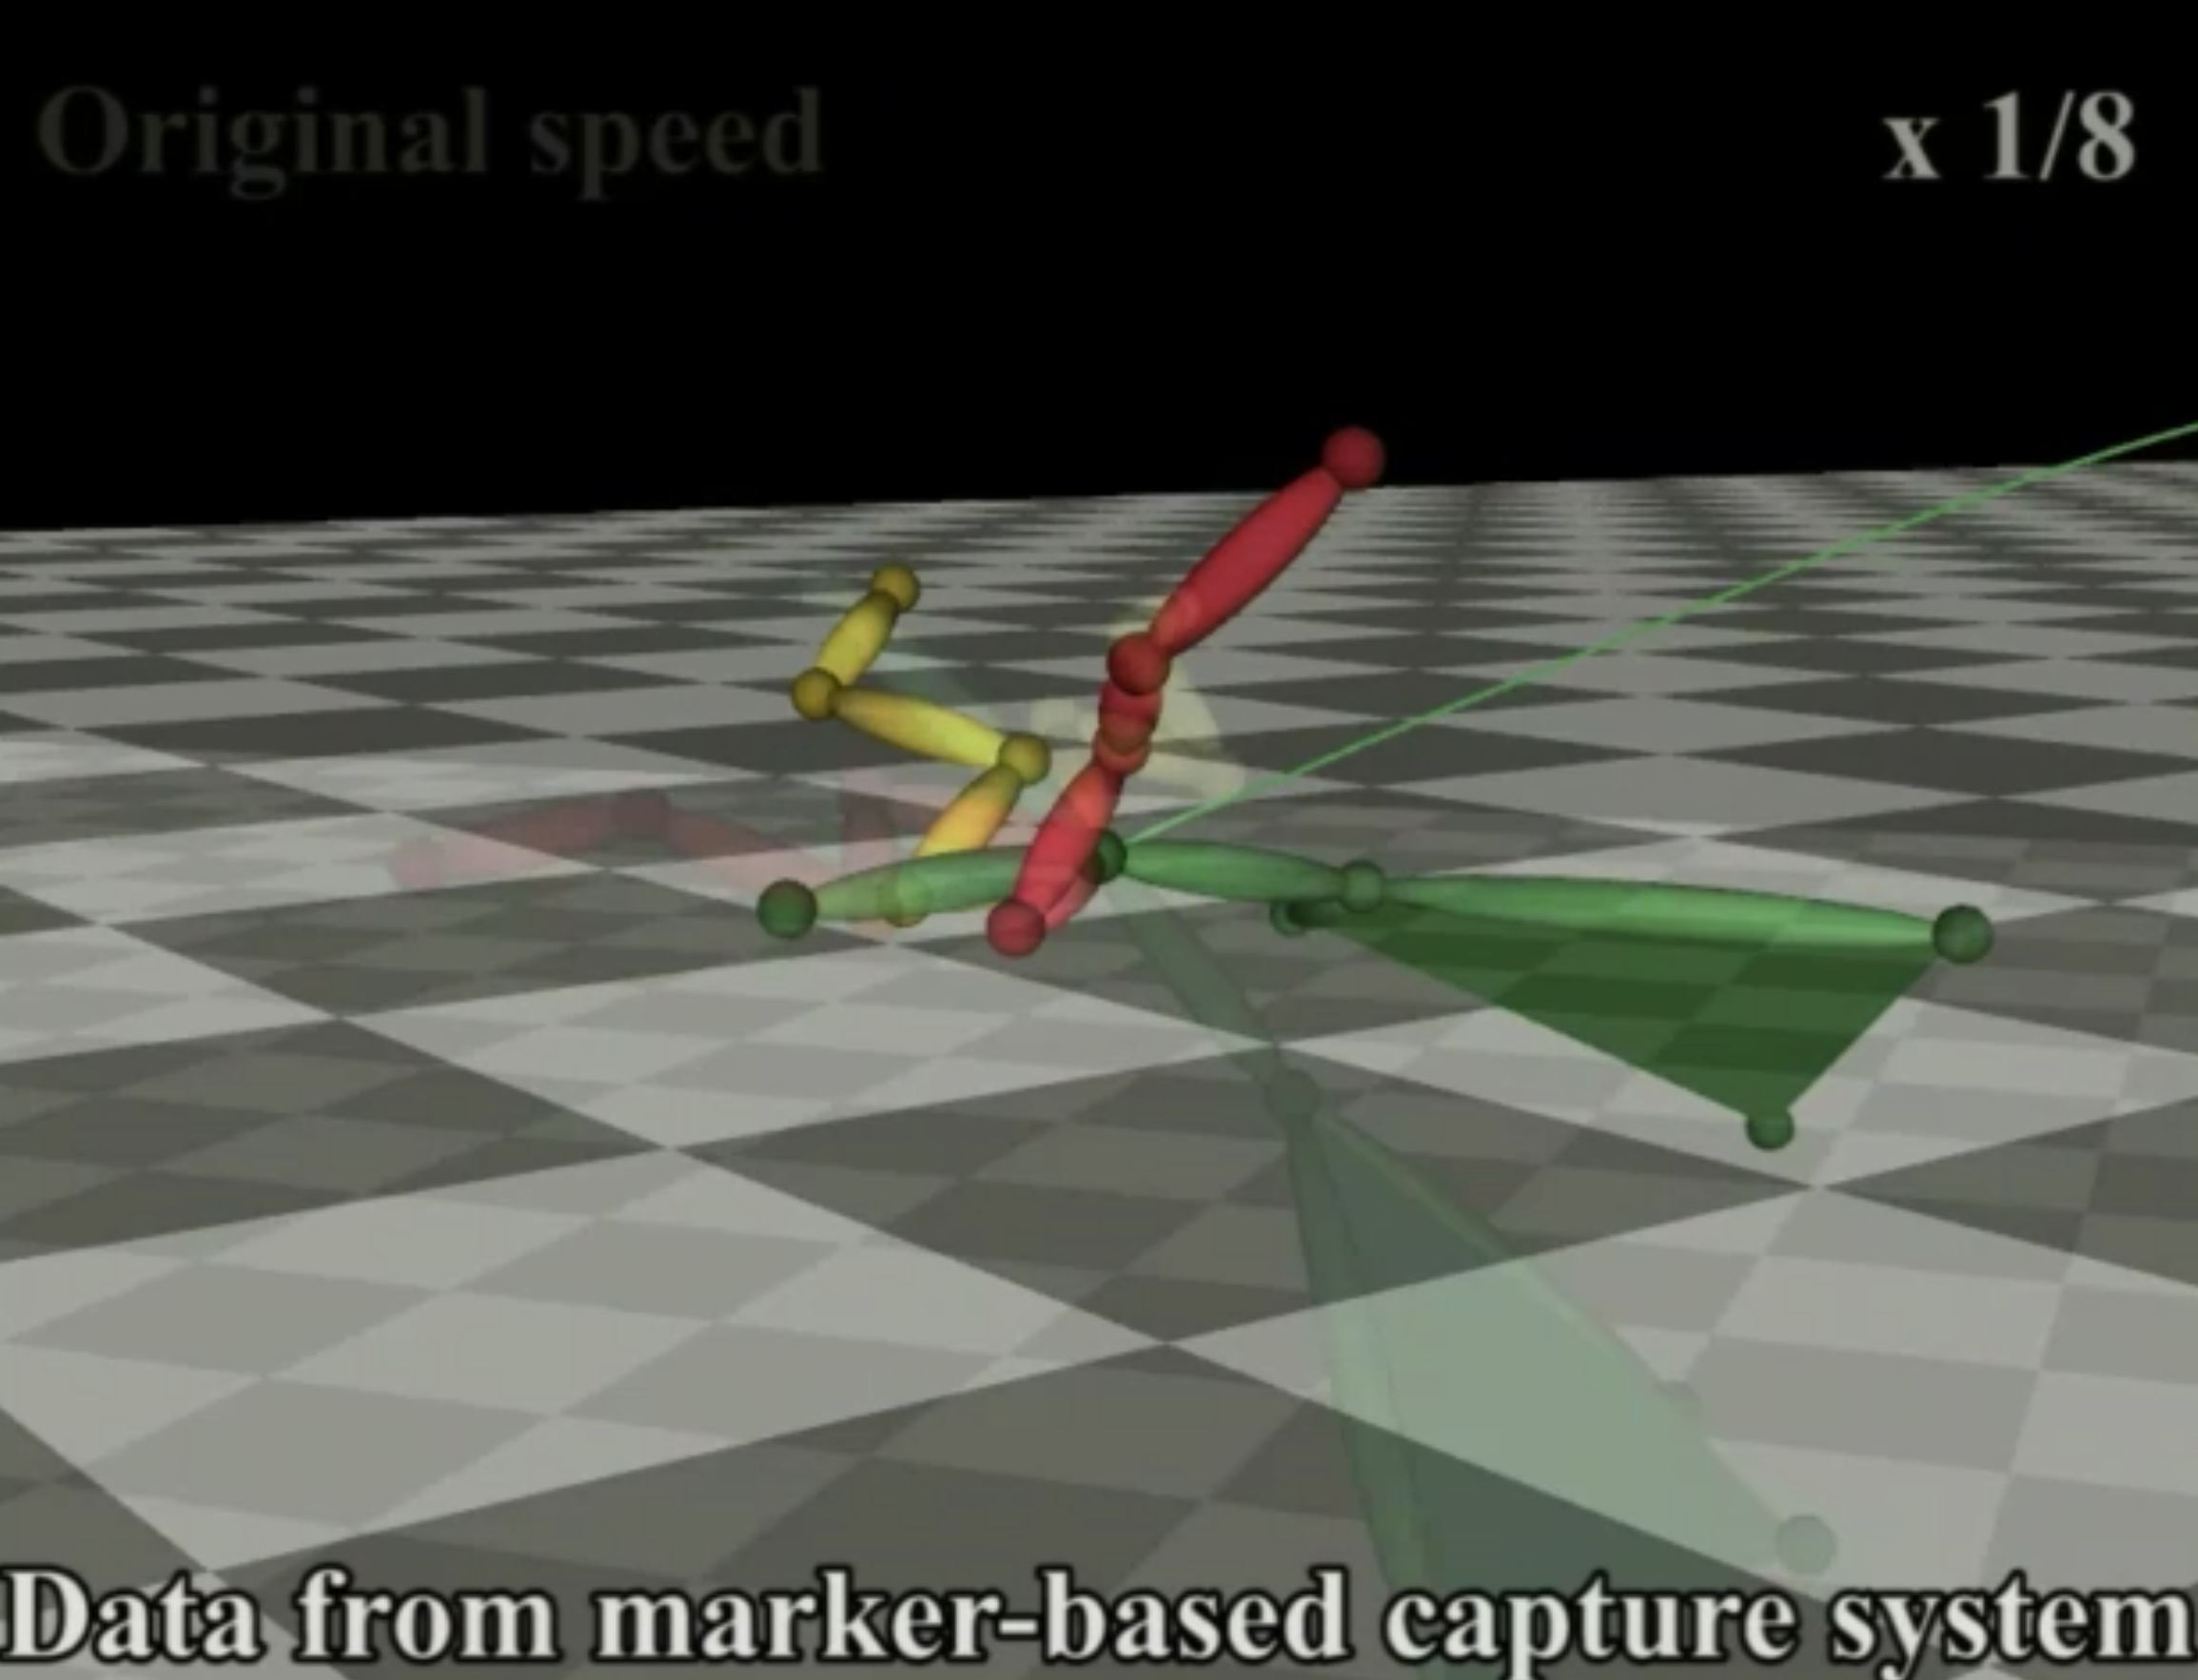
\includegraphics[width=\textwidth]{fileForWriting/model_struct}
			\caption{Joints modeling}
			\label{fig:model_struct}
		\end{subfigure}
	\hfill
		\begin{subfigure}[b]{0.4\textwidth}
			\centering
			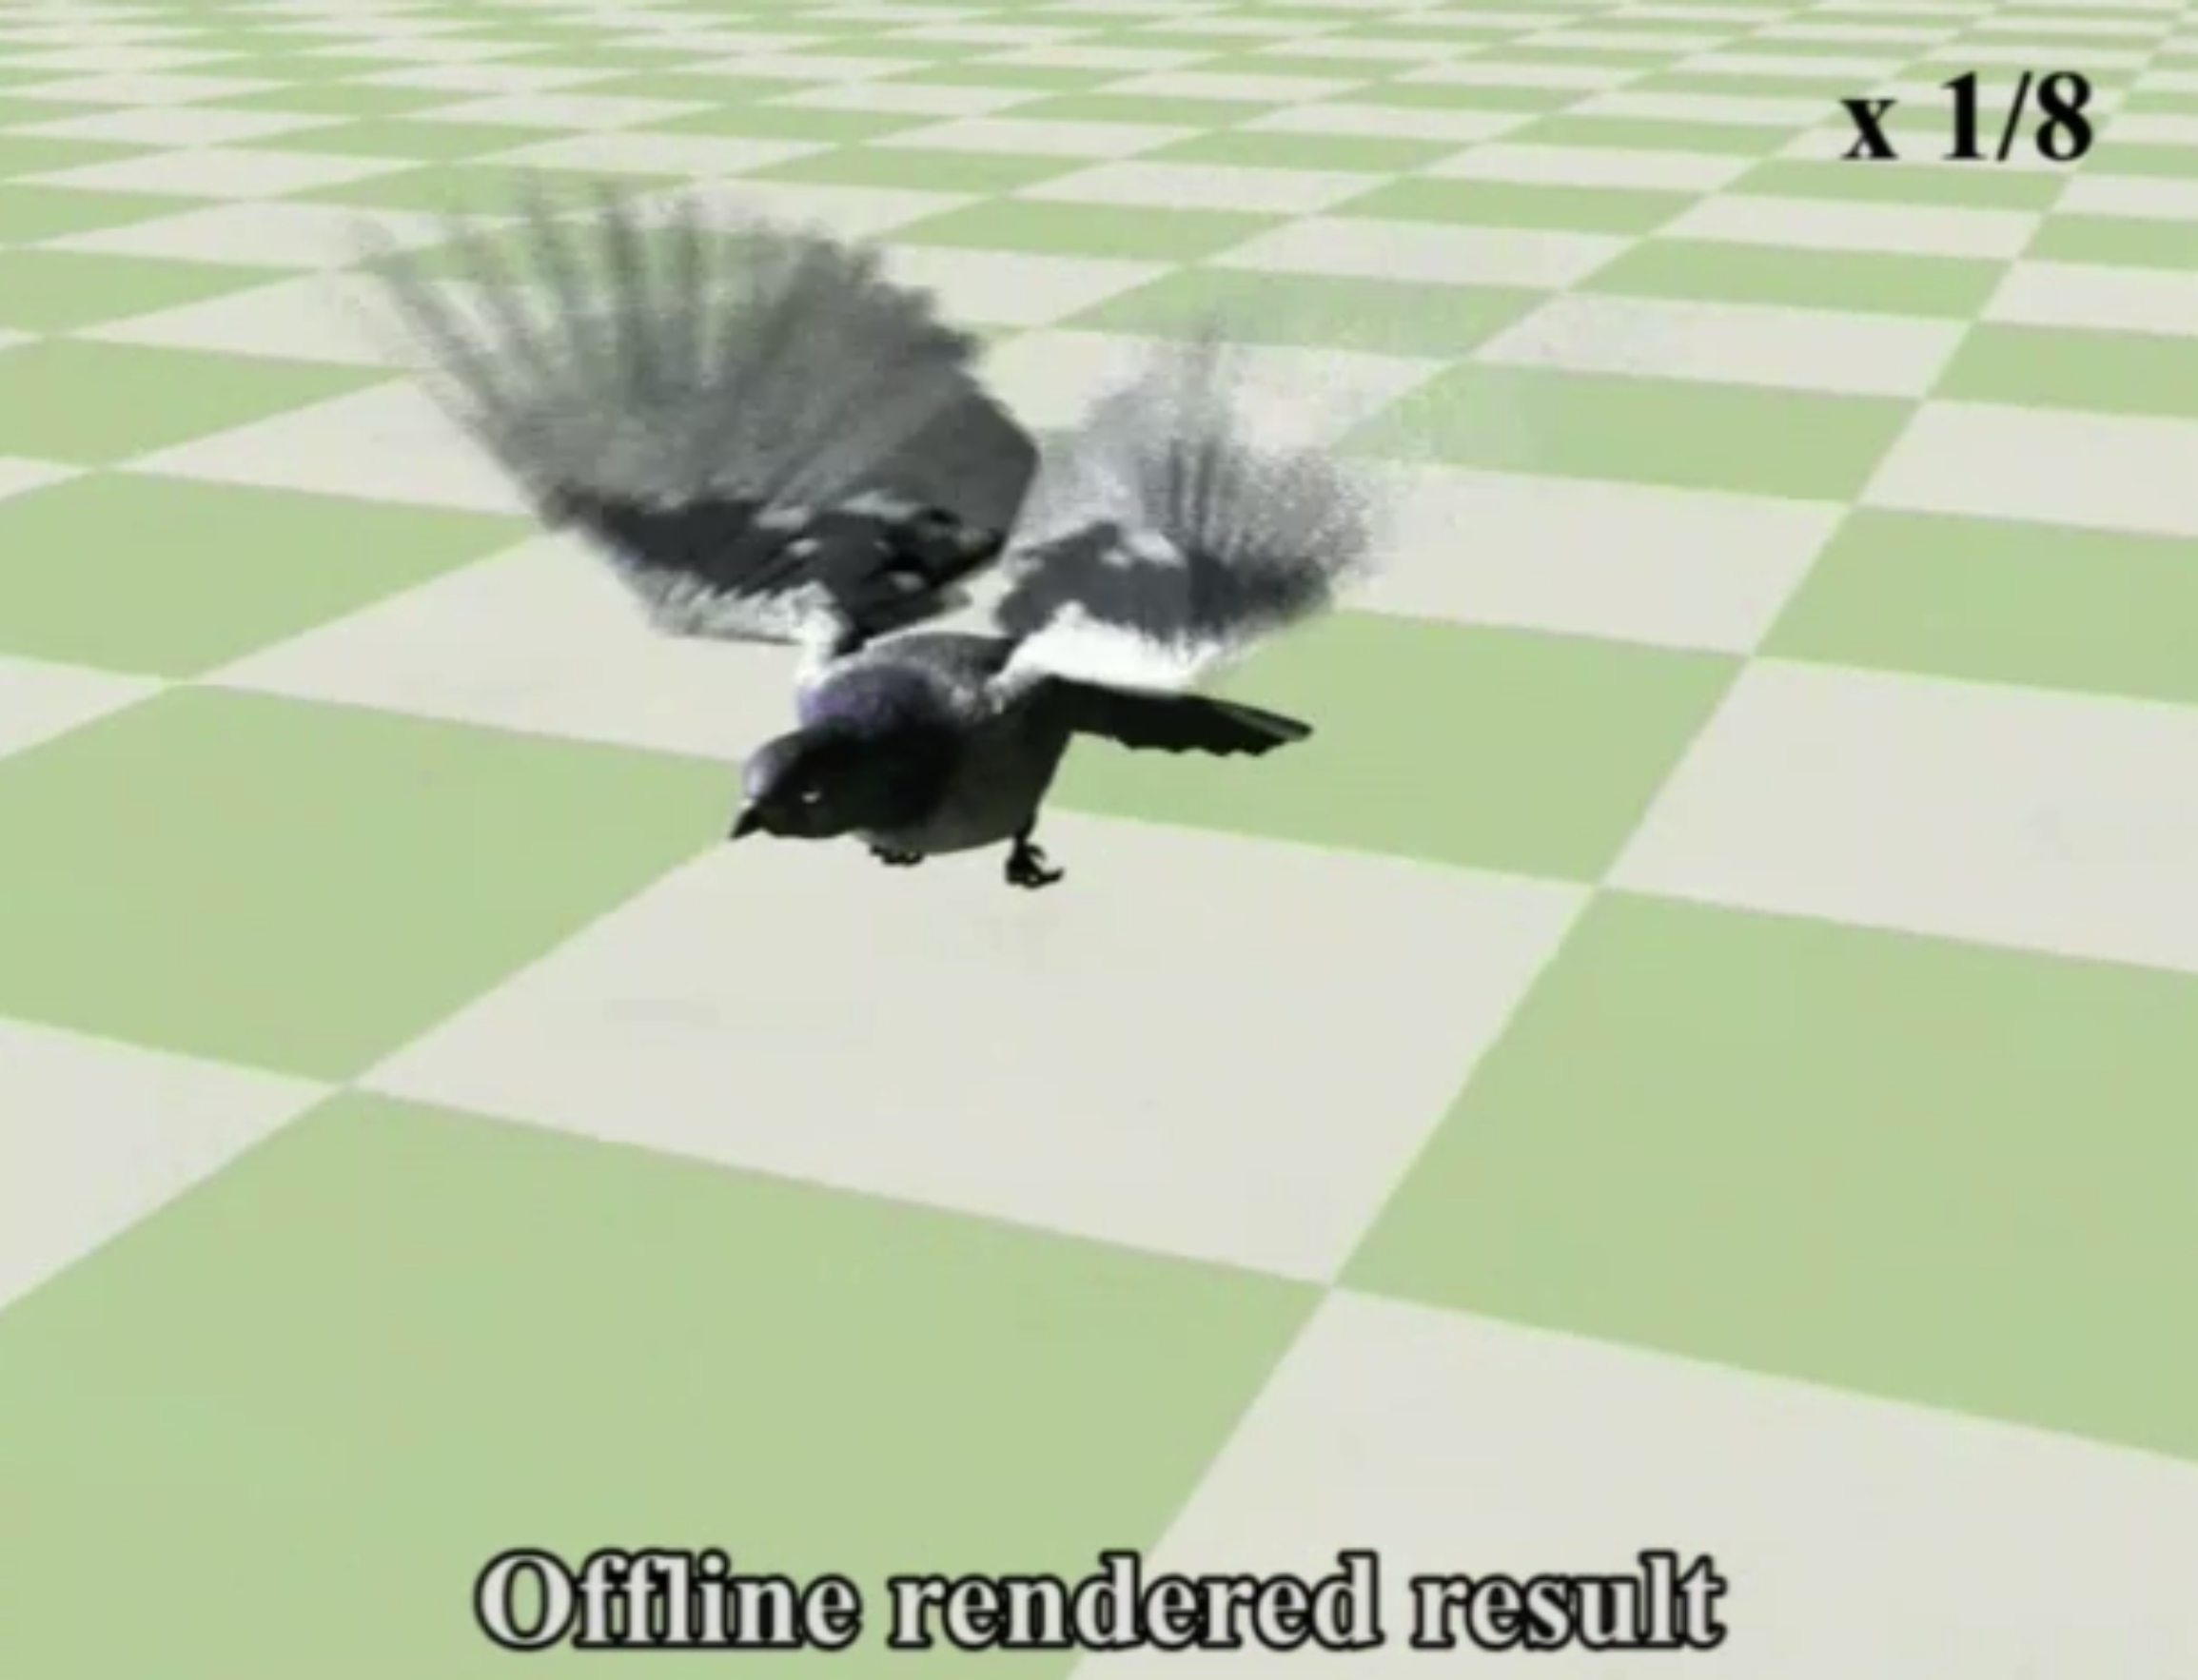
\includegraphics[width=\textwidth]{fileForWriting/model_real}
			\caption{}
			\label{fig:model_real}
		\end{subfigure}
	\caption{Two sample screenshots~\cite{ju_data-driven_2011} for digital twin via a optical motion capture system.}
	\label{fig:system overview}
\end{figure}

%-----------This is a FIGURE-----------------------
\begin{figure}[htbp]
	\centering
	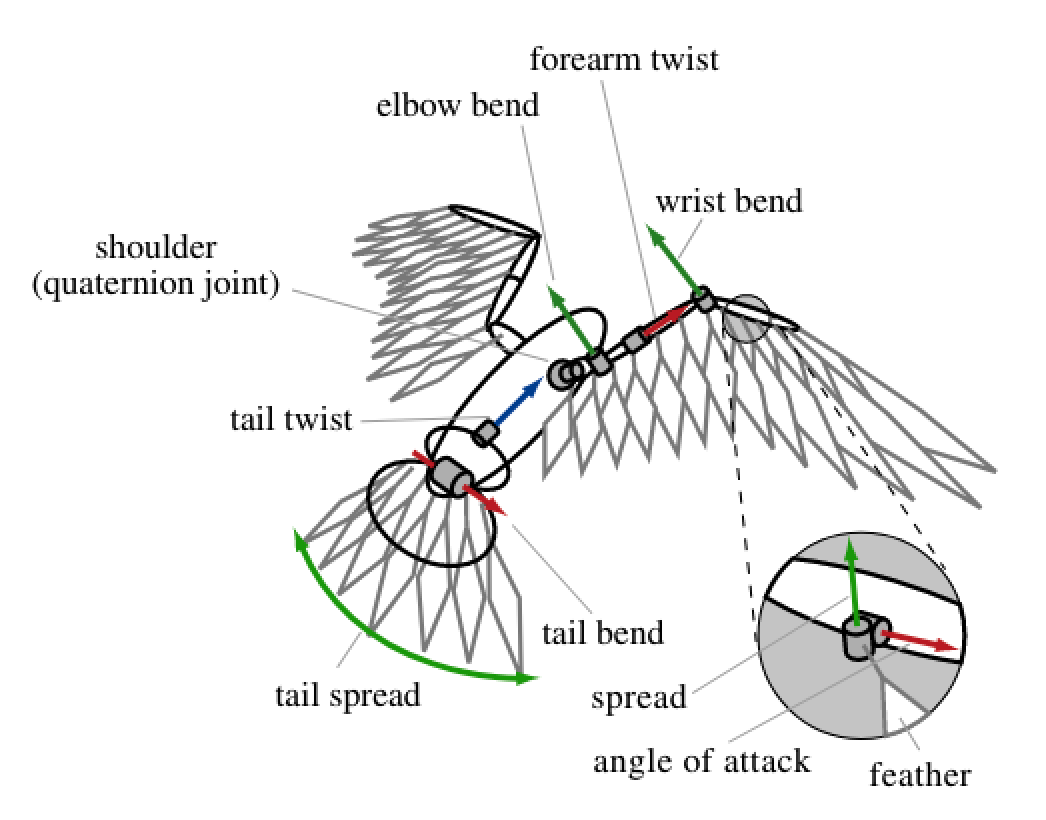
\includegraphics[width=0.5\textwidth]{
		fileForWriting/The bird skeleton}
	\caption{Another bird skeleton for modeling purpose~\cite{wu_realistic_2003}.}
	\label{fig:}
\end{figure}
%--------End of this FIGURE -----------  


To be continued\ldots But one feature is for sure:
there are lots of joints to model, moving the analysis to the next stage.

\newpage
\subsection{Stage \themycounter: Multiple Joints}
\stepcounter{mycounter}
%-----------This is a FIGURE-----------------------
\begin{figure}[htbp]
	\centering
	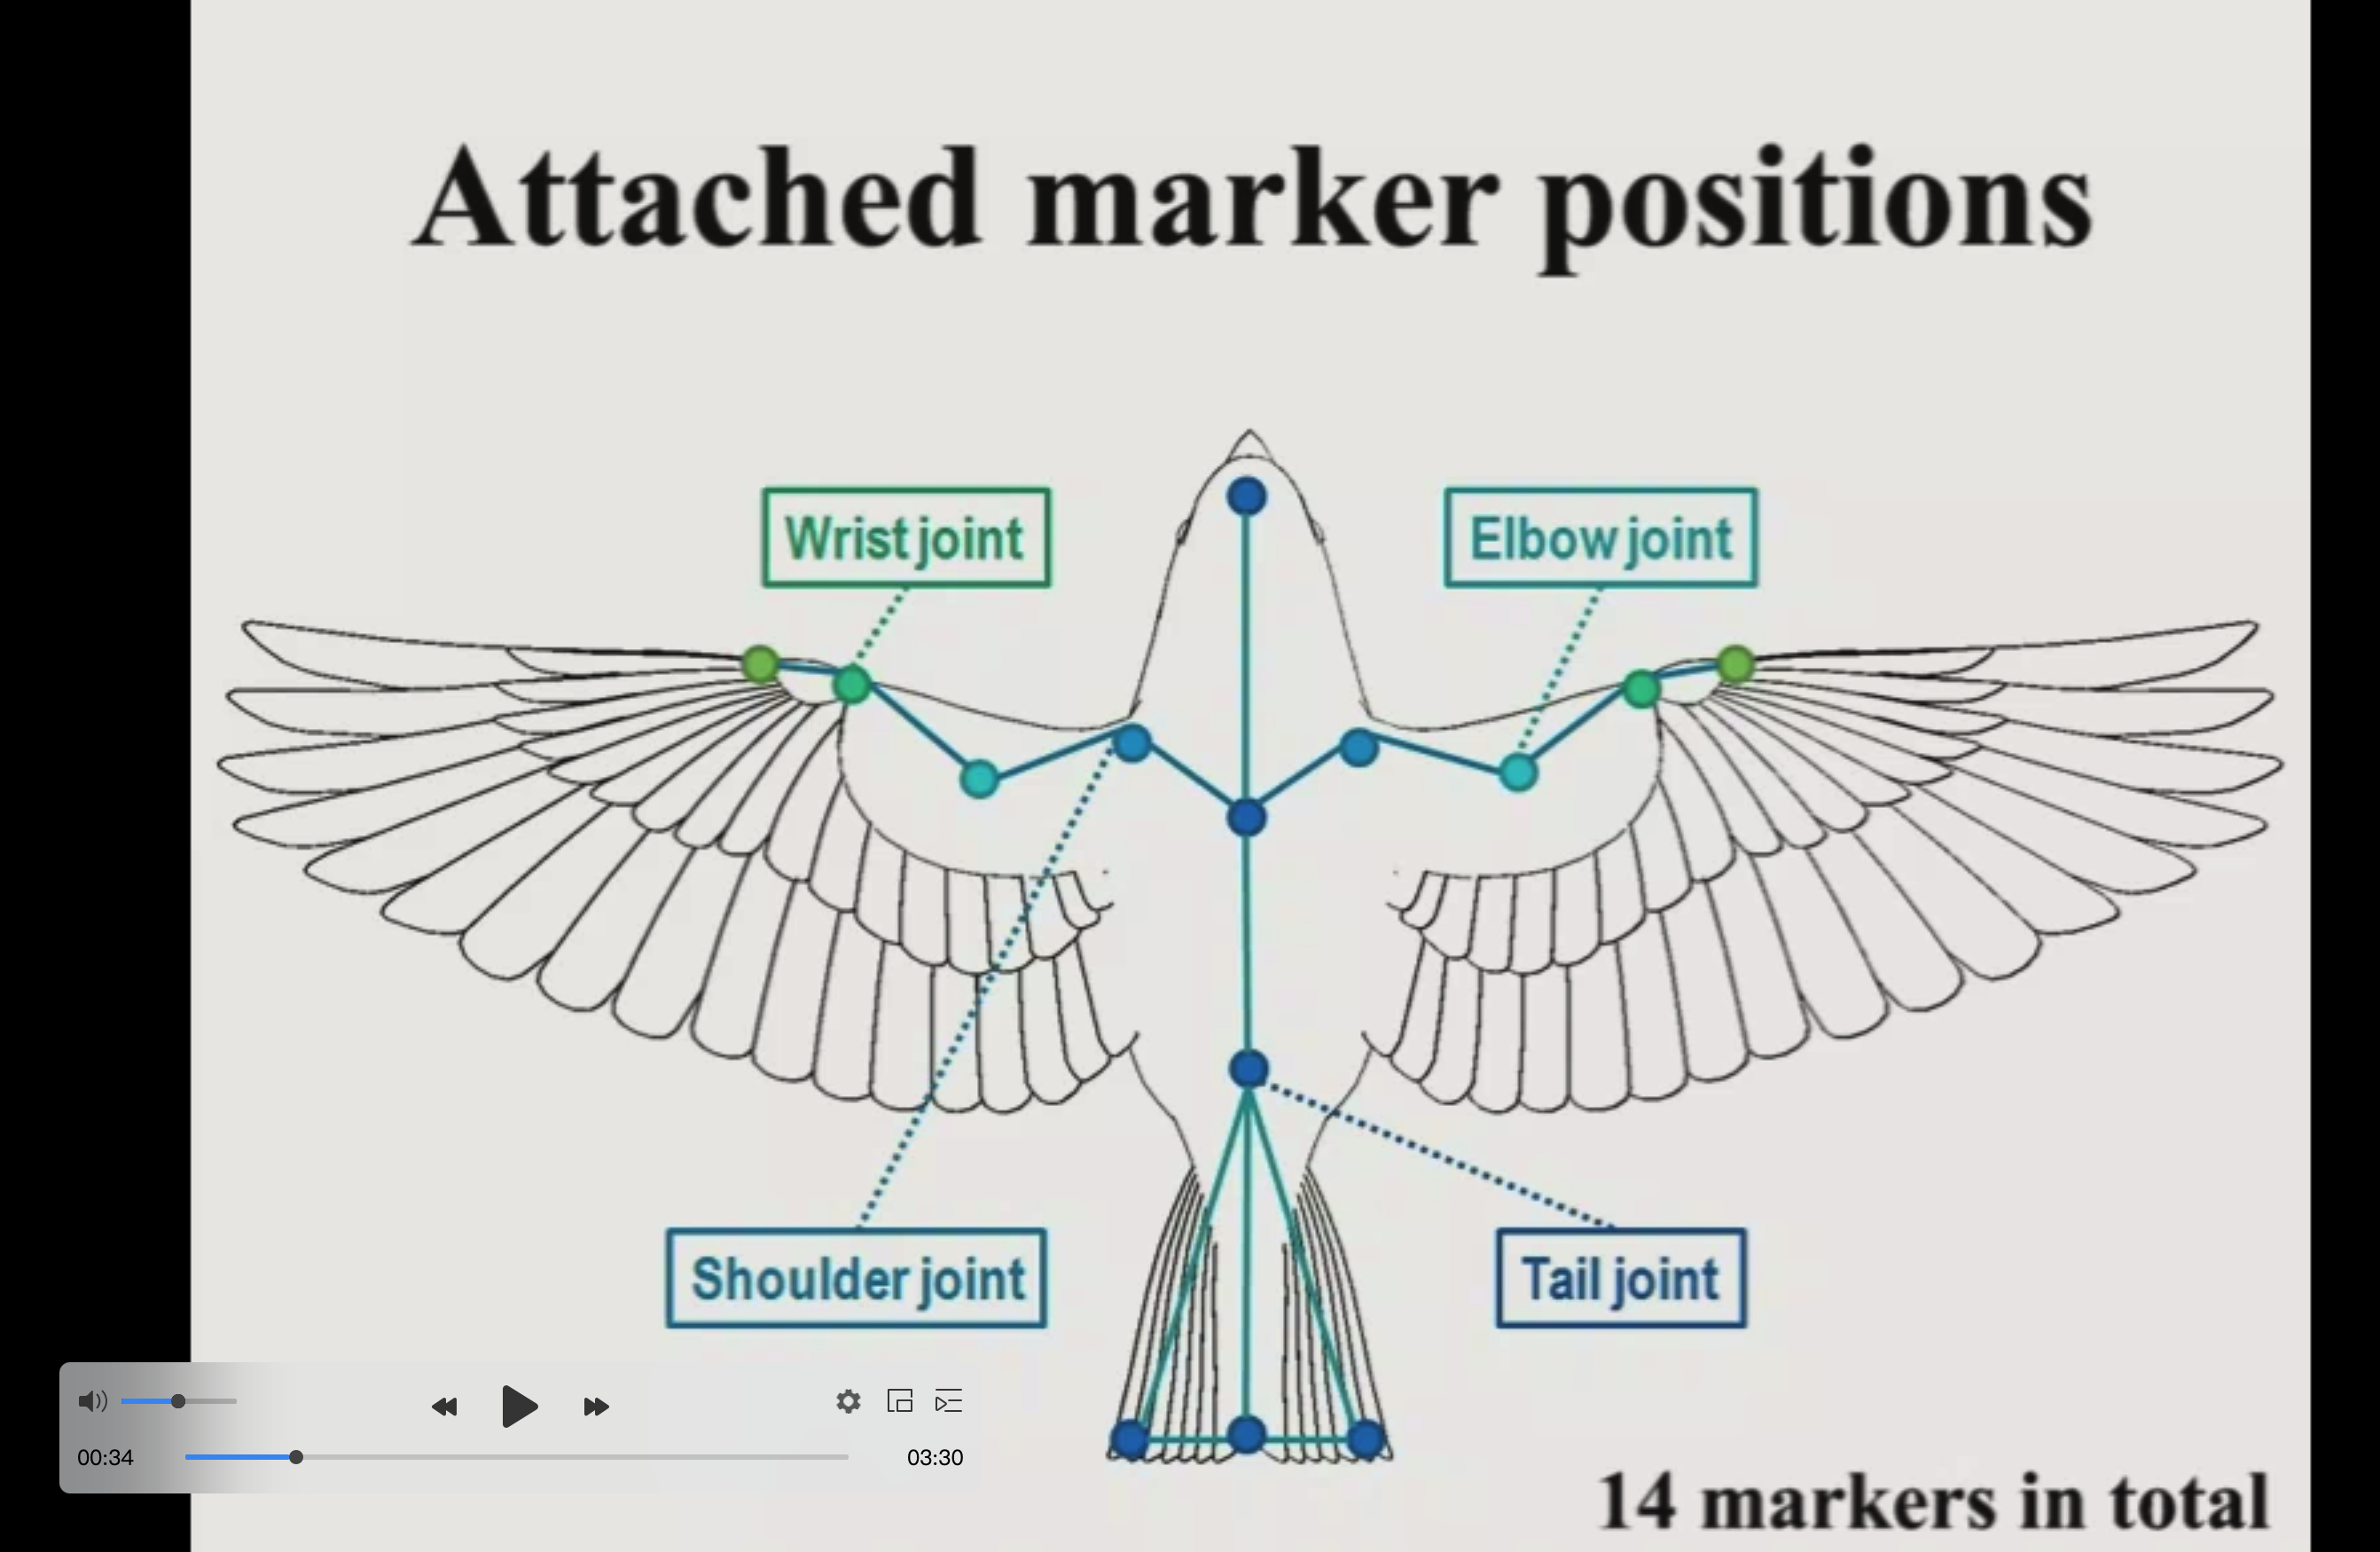
\includegraphics[width=0.8\textwidth]{
		fileForWriting/Data-driven bird simulation}
	\caption{Attached marker positions for optical bio-logging system~\cite{ju_data-driven_2011}, including shoulder, elbow, wrist and tail recordings (240fps). The motion of feathers was also observed by four high speed cameras (1000fps). Proportional Derivative (PD) control approach was used to link two adjacent states detected by the Vicon system.}
	\label{fig:Data-driven Bird Simulation}
\end{figure}
%--------End of this FIGURE -----------  


Figure~\ref{fig:Data-driven Bird Simulation} has demonstrated a data-driven bird simulation through a Vicon optical motion capture system via 14 markers. However, the drawback of such system is the environment limitation since all cameras only focused on a $14\times16\times7(m)$ area.

Hence, one more adaptive method for motion capture is using inertial systems, which requires multiple Inertial Measurement Units (IMUs) to be installed on the target. Given that both motion capture systems have to simulate the model of birds into the monitor, those joints indicated in Figure~\ref{fig:Data-driven Bird Simulation} can be also applied in our Year 2 Project. Therefore, we can limit our attention to stage \themycounter: a simple joint, which will be a basic demo/function. After that, we may try extending it to a more complected target.

\newpage
\subsection{Stage \themycounter: A Simple Joint}
\stepcounter{mycounter}
This stage is mainly about logging the motion of one stick installed with an accelerometer (or with a gyro sensor more). Specifically, we aim to display its movements into the monitor. Discussions will be seperated into hardware and software two parts.

\subsubsection{Hardware Process}

Main components:
\begin{enumerate}
    \item IMU 3DOF/6DOF/9DOF Board (IIC/SPI interface)
    \item Microcontroller including AHRS lib
    \item Power supply.
\end{enumerate}
%https://uk.farnell.com/dfrobot/sen0250/i2c-6-axis-motion-sensor-arduino/dp/3517944?st=imu
%https://uk.farnell.com/digilent/410-326/pmod-board-9-axis-imu-plus-barometer/dp/2726217?st=imu
%https://uk.farnell.com/stmicroelectronics/steval-mki193v1/adapter-board-mems-adapter-motherboard/dp/3126311?st=imu

\noindent
Procedures
\begin{enumerate}
    \item Sensor calibration \& compensation
    \item Transform raw data to roll\&yaw\&pitch using a AHRS lib
    \item Send the data package to PC via Virtual Serial Port, which has a high speed
\end{enumerate}

\subsubsection{Software Process}
\noindent
Software Tools:
\begin{enumerate}
    \item Browser with WebGPU/WebGL API: three.js
\end{enumerate}
\noindent
Procedures: modeling \& displaying

\begin{enumerate}
    \item Create a cuboid in https://threejs.org/editor/.
    \item Make a point static and lock the shape.
    \item Link the position of another point to an input file, which stores the coordinates of points.
\end{enumerate}

\noindent
Procedures: data processing
\begin{enumerate}
	\item Receive roll\&yaw\&pitch data from the microcontroller.
	\item Format\&interpolate the data to the file for modeling.
\end{enumerate}

%%%%%%%%%%%%%%%%%%%%%%%%%%%%%%%%%%%%%%%%%%%%%%%%%%%%%%%%%%%%%%%%%%%%%%%%%%%%%%%%%%%%%%%%%%%%%%
%Schedule
%%%%%%%%%%%%%%%%%%%%%%%%%%%%%%%%%%%%%%%%%%%%%%%%%%%%%%%%%%%%%%%%%%
\newpage
\section{Schedule}
Below is a draft schedule for the first two weeks, namely developing hardware and software separately. If successful in these two weeks, we will then combine the two systems together and test it in the last two weeks. Our lab location is \textbf{ROOM302, 7A-7D}.
\subsection{Week-1 \& Week-2}


\subsubsection{Hardware System}


\begin{table}[!ht]
	\centering
	\caption{Task allocation for hardware system in the first two weeks}
	\begin{tabular}{|l|l|l|}
		\hline
		& Compulsory Task             & Optional Task                        \\ \hline
		Brissenden, Jack        & \multirow{2}{*}{T0, T1, T2} & \multirow{2}{*}{T4(not-yet-decided)} \\ \cline{1-1}
		Guo, Jiajun             &                             &                                      \\ \hline
		Canning, Charles Thomas & T3                          & T0, T1, T2                           \\ \hline
	\end{tabular}
	\label{tab:hardware_group}
\end{table}

\textbf{Task-0: pre-work} 	[EASY]
\begin{enumerate}
    \item collect \& check the components.
    \item prepare cables for linking.
\end{enumerate}

\textbf{Task-1: single IMU} 	[EASY]
\begin{table}[!ht]
	\centering
	\caption{Time-schedule for T1-``single IMU''}
	\begin{tabular}{|c|c|}
		\hline
		Early-finish-date & Thursday Evening of W1 \\ \hline
		Late-finish-date & Friday Evening of W1 \\ \hline
	\end{tabular}
	\label{tab:HD_TASK_1}
\end{table}

\begin{enumerate}
	\item construct one circuit with only one IMU, excluding IIC multiplexer.
	\item initialize the IMU (if not) !
	\item fetch data from this single IMU and then convert them into roll/yaw/pitch (if needed), output them in the terminal.
\end{enumerate}

%-----------This is a FIGURE-----------------------
\begin{figure}[htbp]
	\centering
	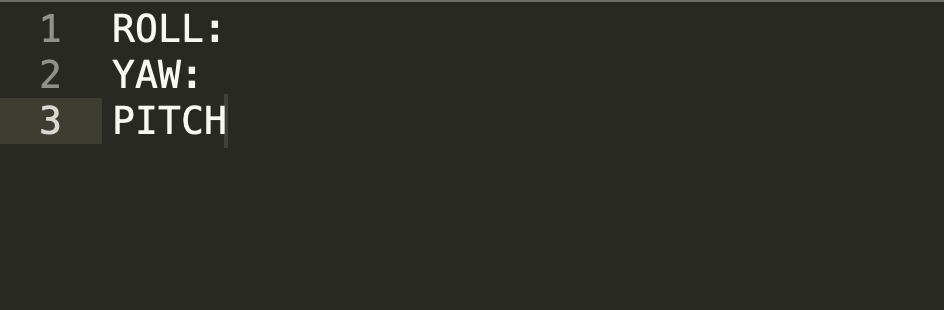
\includegraphics[width=0.5\textwidth]{
		fileForWriting/OUTPUT_FORMAT_T1}
	\caption{Output format for T1}
	\label{fig:OUTPUT_FORMAT_T1}
\end{figure}
%--------End of this FIGURE -----------


\textbf{Task-2: multiple IMUs} 	[Half-difficult]
\begin{table}[!ht]
	\centering
	\caption{Time-schedule for T2-``multiple IMUs''}
	\begin{tabular}{|c|c|}
		\hline
		Early-finish-date & Friday Evening of W1 \\ \hline
		Late-finish-date & Monday Morning of W2 \\ \hline
	\end{tabular}
	\label{tab:HD_TASK_2}
\end{table}

\begin{enumerate}
	\item construct the circuit including the IIC multiplexer, namyly multiple IMUs.
	\item initialize the IMUs (if not)!
	\item fetch data from those IMUs and then convert them into roll/yaw/pitch (if needed), output them in terminal with their corresponding IMUs' index.
\end{enumerate}

%-----------This is a FIGURE-----------------------
\begin{figure}[htbp]
	\centering
	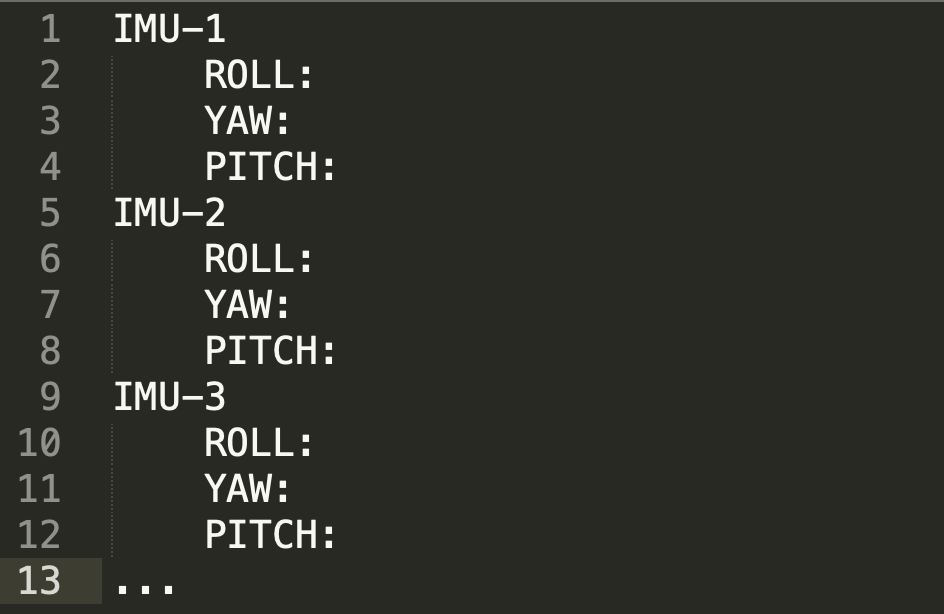
\includegraphics[width=0.5\textwidth]{
		fileForWriting/OUTPUT_FORMAT_T2}
	\caption{Output format for T2}
	\label{fig:OUTPUT_FORMAT_T2}
\end{figure}
%--------End of this FIGURE -----------

\textbf{TASK-3: communicate with PC using Berkeley Socket} 	[Difficult] [Primary-Plan]

\begin{table}[!ht]
	\centering
	\caption{Time-schedule for T3-``Berkeley Socket''}
	\begin{tabular}{|c|c|}
		\hline
		Early-start-date & Thursday of W1 \\ \hline
		Late-start-date & Friday of W1 \\ \hline
		Early-finish-date & Wednesday of W2 \\ \hline
		Late-finish-date & Monday of W3 \\ \hline
	\end{tabular}
	\label{tab:HD_TASK_3}
\end{table}

\begin{enumerate}
	\item Board Type: Arduino-WIFI-Rev2.
	\item support sending HTTP-POST request.
\end{enumerate}

\textbf{TASK-4: communicate with PC using USART} 	[Half-difficult] [Backup-Plan for TASK-3]
\begin{table}[!ht]
	\centering
	\caption{Time-schedule for T4-``USART''}
	\begin{tabular}{|c|c|}
		\hline
		Start-date & not-yet-decided \\ \hline
		End-date & not-yet-decided \\ \hline
	\end{tabular}
	\label{tab:HD_TASK_4}
\end{table}

\begin{enumerate}
	\item Board Type: Arduino-Nano.
	\item support USART transmitting.
\end{enumerate}

\newpage
\subsubsection{Software System}


\begin{table}[!ht]
	\centering
	\caption{Task allocation for software system in the first two weeks}
	\begin{tabular}{|l|l|l|}
		\hline
		~ & Compulsory Task & Optional Task \\ \hline
		Shen, Yixiao & T1, T2 & T3(not-yet-decided) \\ \hline
		Zhou, Qi & T1, T2 & T3(not-yet-decided) \\ \hline
	\end{tabular}
	\label{tab:software_group}
\end{table}

\textbf{TASK-1: build a simple socket server using C++ on LinuxOS.}     [EASY] [Half-completed]
\begin{enumerate}
    \item support responding HTTP-GET request.	[Bug: missing of MIME Type]
    \item support forward one message from one client(Arduino) to another client(browser). [Wait for Hardware-TASK-3]
    \item support responding HTTP-POST request. [Wait for Hardware-TASK-3]
\end{enumerate}

\textbf{TASK-2: build a simple displaying engineer using three.js on Web, namely HTML\&CSS\&JS.}
\begin{table}[!ht]
	\centering
	\caption{Time-schedule for T2-``displaying engineer''}
	\begin{tabular}{|c|c|}
		\hline
		Early-finish-date & Monday morning of W2 \\ \hline
		Late-finish-date & Friday of W2 \\ \hline
	\end{tabular}
	\label{tab:SD_TASK_2}
\end{table}


\begin{enumerate}
	\item bind joints model with their corresponding IMUs. 	[Difficult]	[Need more discussion]
need more discussions here.
	\item support input from server.	[Interface defined]
\end{enumerate}

\textbf{TASK-3: support serial port communication.}  [Half-Difficult] [Backup-Plan for Hardware-TASK-3]
\begin{table}[!ht]
	\centering
	\caption{Time-schedule for T3-``serial port''}
	\begin{tabular}{|c|c|}
		\hline
		Start-date & not-yet-decided \\ \hline
		Finish-date & not-yet-decided \\ \hline
	\end{tabular}
	\label{tab:SD_TASK_3}
\end{table}


%%%%%%%%%%%%%%%%%%%%%%%%%%%%%%%%%%%%%%%%%%%%%%%%%%%%%%%%%%%%%%%%%%%%%%%%%%%%%%%%%%%%%%%%%%%%%%
%Relevant Articles
%%%%%%%%%%%%%%%%%%%%%%%%%%%%%%%%%%%%%%%%%%%%%%%%%%%%%%%%%%%%%%%%%%
\newpage
\section{Relevant Articles}

\begin{enumerate}
	\item A optical bio-loggers for birds~\cite{ju_data-driven_2011}.
	\item A simple 3-axial accelerometer bio-loggers for birds~\cite{taylor_birds_2019}.
    \item A simple 3-axial accelerometer bio-loggers for cats~\cite{watanabe_new_2005}.
    \item A simple 3-axial accelerometer bio-loggers for imperial cormorants~\cite{gomez_laich_identification_2009}.
    \item Leonardo da Vinci’s discovery of the dynamic soaring by birds in wind shear~\cite{richardson_leonardo_2019}.
    \item Wind Energy Extraction by Birds and Flight Vehicles~\cite{lissaman_wind_2005}.
    \item Automatically generating holograms via accelerators~\cite{sakamoto_can_2009}.
\end{enumerate}









%%%%%%%%%%%%%%%%%%%%%%%%%%%%%%%%%%%%%%%%%%%%%%%%%%%%%%%%%%%%%%%%%%%%%%%%%%%%%%%%%%%%%%%%%%%%%%
%References & Appendix
%%%%%%%%%%%%%%%%%%%%%%%%%%%%%%%%%%%%%%%%%%%%%%%%%%%%%%%%%%%%%%%%%%
\newpage
\bibliographystyle{IEEEtran}
\bibliography{references}
\addcontentsline{toc}{section}{References}

\end{document}
